\documentclass{article}
\usepackage{mathmag}

\usepackage{amsmath,amsthm}
\usepackage{graphicx}
\usepackage{hyperref}
\usepackage{url}
\usepackage{amsfonts}

\usepackage{multicol}


% NOTE mathmag.sty calls the text fonts. For this template we are using times.sty
% from the standard LaTeX distribution.

%% IF YOU HAVE FONTS INSTALLED you can use these math fonts to more
%% closely approximate the final product.
%\usepackage{mtpro2}
%\usepackage{mathtime}

\theoremstyle{theorem}
\newtheorem{theorem}{Theorem}

\theoremstyle{definition}
\newtheorem*{definition}{Definition}
\newtheorem*{remark}{Remark}

\allowdisplaybreaks

\makeatletter
\@addtoreset{footnote}{page}
\makeatother

%%%%%%%%%%%%%%%%%%%%%%%%%%%%%%%%%%%%%%%%%%%%%%%%%%
\begin{document}

\title{Segregation Surfaces}

\author{Author Name\\               %%%% Leave ALL of these as is in your initial submission
\scriptsize affiliation line 1\\    %%%% to allow for double blind reviewing.
affiliation line 2\\                %%%% They should be filled in when you are submitting
email address}                      %%%% your final manuscript.

\maketitle

\noindent Over the past half century, social scientists have devised a clever assortment of tools to measure the nature and extent of segregation. \cite{harrisjohnson18} Usually, a segregation measurement takes the form of a number, or \textit{index}, which quantifies the isolation and clustering of groups defined by race, income, education, or other factors. Numerical indices are handy because they can give us ways to track changes in a neighborhood over time, and they allow for comparisons among different regions.

However, segregation usually takes place on a map, not on a number line. Numerical summary statistics alone are limited when it comes to discerning geometric patterns in two-dimensional data. In this note, we use some familiar ideas from third-semester calculus to extend the machinery behind some commonly-used segregation indices. Segregation can be represented by a surface, and the geometric properties of these surfaces can help us see how our cities and towns are divided.

\section{Numerical measures of segregation.}

D, checkerboard problem.

Spatial measures. Reardon \cite{reardonosullivan04}, Wong.

\section{Drawing segregation boundaries.}

Redefine fhat using bayes theorem. Motivate by simulated example.

In practice, the functions $a$, $s$, and $f$ must be estimated from data. [kernel smoothing] \cite{wandjones11}

Look at some examples of outlines

TODO: Graphic showing over/under fitting. Baltimore?

\begin{figure}
  \includegraphics{overunderfit.pdf}
  \caption{Fifty-percent contours of $\hat{f}$ for three choices of smoothing parameters. The left plot shows oversmoothing, while the right plot shows undersmoothing.}
  \label{fig:overunderfit}
\end{figure}

\section{The segregation gradient.}

County analysis

The average magnitude of the gradient is moderately correlated ($r \approx 0.6$) with Reardon and O'Sullivan's exposure/isolation index $\tilde{P}*$ and weakly correlated ($r\approx 0.3$) to their spatial information theory index $\tilde{H}$.

Scatterplot? exposure vs maggrad? Group 1 to group 2 exposure is 1-segp2. Plot vs. seg2Di and look at patterns/outliers.

Colored gradient: sharper boundaries.

Gradient arrows; obstruction detection.

\begin{figure}
  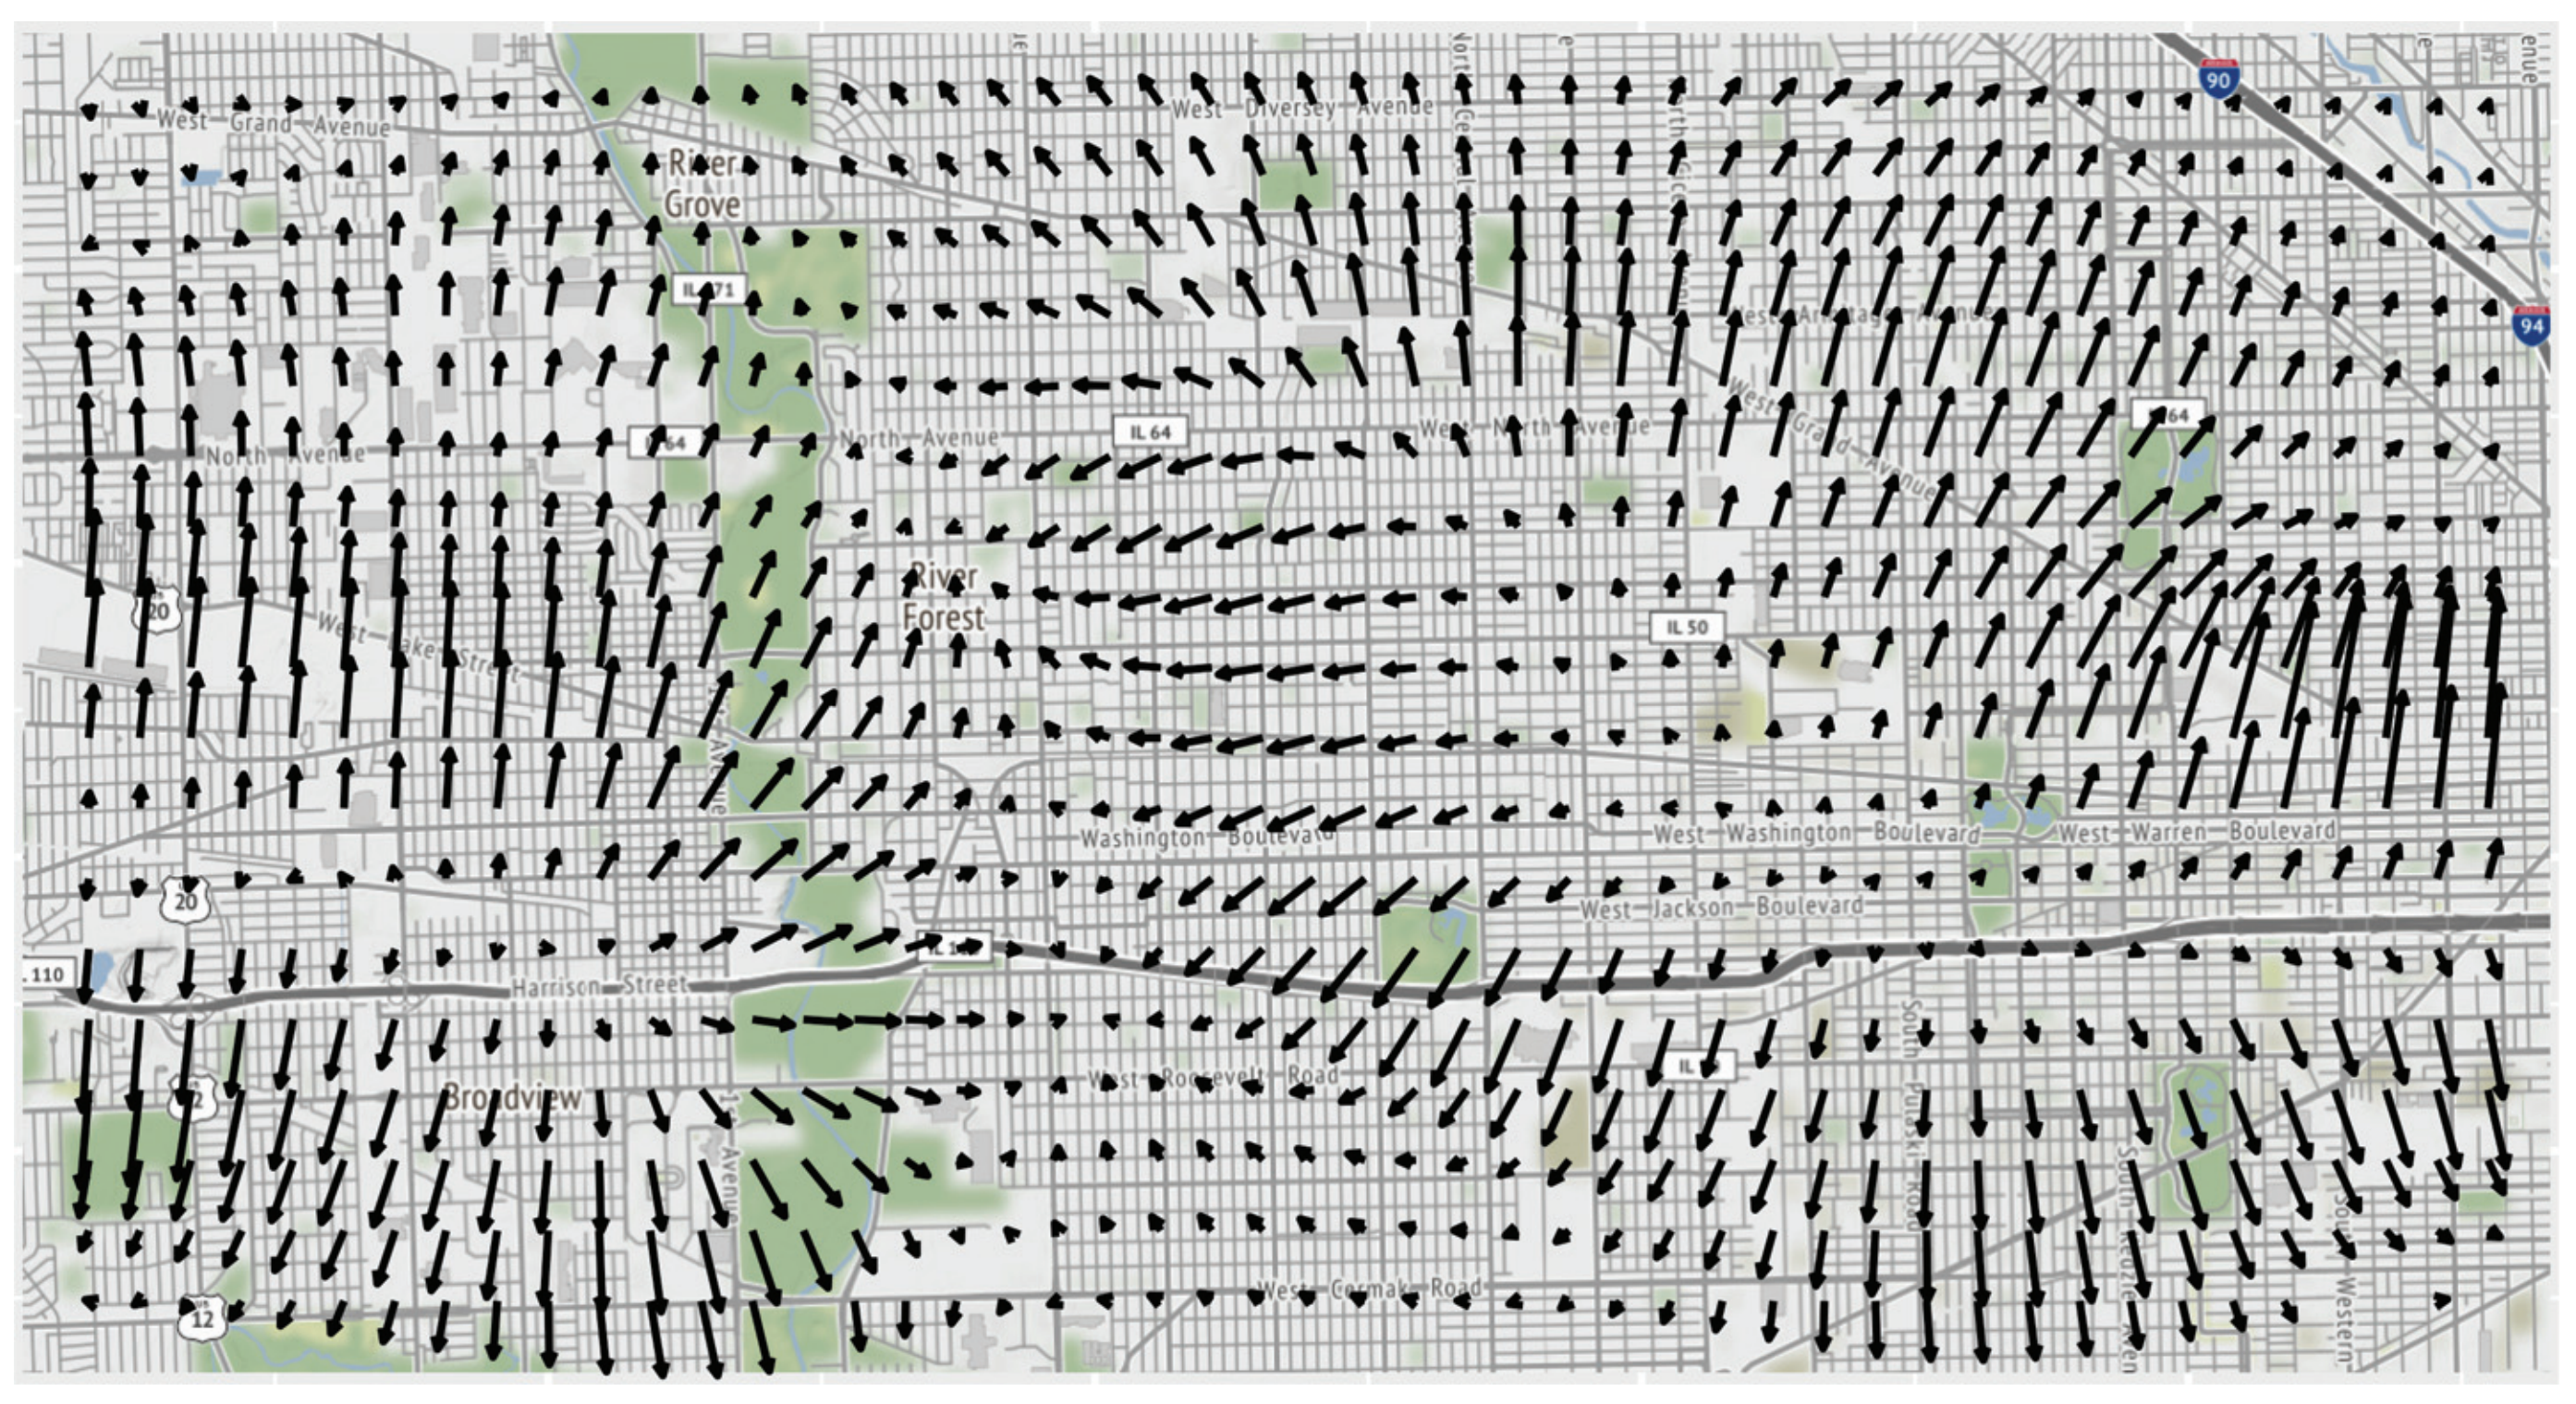
\includegraphics{chicagowest.pdf}
  \caption{White/non-white segregation gradients in the near-west suburbs of Chicago.}
  \label{fig:chicagowest}
\end{figure}

\begin{figure}
  \includegraphics{sanfran1317.pdf}
  \caption{Gentrification in San Fransisco. Income segregation patterns have changed from 2013 (left) to 2017 (right). The contours enclose neighborhoods whose residents tend to have incomes below the county median. Some of these neighborhoods have been shrinking. Thicker contours represent starker divisions.}
  \label{fig:sanfran1317}
\end{figure}


\begin{thebibliography}{3}

\bibitem{harrisjohnson18}
Harris, R., Johnson, R. (2018). Measuring and modelling segregation---New concepts, new methods and new data. \textit{Environment and Planning B: Urban Analytics and City Science.} 45(6): 999--1002. doi:\href{http://dx.doi.org/10.1177/2399808318808889}{10.1177/2399808318808889}

\bibitem{reardonosullivan04}
Reardon, S., O'Sullivan, D. (2004). Measures of Spatial Segregation. \textit{Sociological Methodology.} 34: 121--162. doi:\href{http://dx.doi.org/10.1111/j.0081-1750.2004.00150.x}{10.1111/j.0081-1750.2004.00150.x}

\bibitem{wandjones11} Wand, M. P., Jones, M. C. (2011). \textit{Kernel smoothing}, London: Chapman \& Hall.

\end{thebibliography}

\end{document}
